\documentclass{article}
\usepackage{graphicx} % Pro vkládání obrázků
\usepackage{hyperref} % Pro křížové odkazy a odkazy
\usepackage{booktabs} % Pro lepší formátování tabulek
\usepackage{titlesec} % Pro nastavení sekcí
\usepackage{xcolor} % Pro barevný text
\usepackage{polyglossia} % Pro podporu češtiny
\usepackage[backend=bibtex,style=numeric,citestyle=numeric,sorting=none]{biblatex} % Pro správné formátování citací
\usepackage[a4paper,margin=2.5cm]{geometry} % Nastavení okrajů
\setdefaultlanguage{czech} % Nastavení jazyka na češtinu
\addbibresource{bibliografie.bib} % Přidání bibliografie

% Nastavení, aby každá sekce začínala na nové stránce
\newcommand{\sectionbreak}{\clearpage}
\titlespacing*{\section}{0pt}{0pt}{0pt}
\titlespacing*{\sectionbreak}{0pt}{0pt}{0pt}

% Vlastní příkazy s parametry
\newcommand{\highlight}[2]{\textbf{\textcolor{#1}{#2}}}
\newcommand{\point}[1]{\noindent \textbf{#1:}}

\title{PTY semestrální práce}
\author{Martin Šimon}
\date{Prosinec 2024}

\begin{document}

\maketitle

\pagenumbering{gobble} % Vypnutí číslování na první stránce

\tableofcontents
\pagenumbering{arabic} % Zapnutí číslování od druhé stránky
\setcounter{page}{2}

\clearpage

\section{Úvod}
Tento dokument je vytvořen jako semestrální práce pro kurz PTY. V tomto dokumentu budou texty vzané z 
maturitní četby z knihy Farma zvířat od George Orwella a následně také některé texty z bakalářského projektu.

\section{George Orwell}

\subsection{Život George Orwella}

Byl britský novinář, esejista a spisovatel, který žil v letech 1903–1950. Vlastním jménem Eric Arthur Blair. Psal pod pseudonymem, skutečné jméno Erik Blér. Narodil se v Indii, kde pracoval jeho otec jako úředník. Když měl 1~rok, matka ho odvezla do Anglie. Měl dvě sestry. Vystudoval soukromou střední školu, ale jelikož mu rodiče nemohli platit studium na univerzitě, začal pracovat. Nějakou dobu žil „na ulici“ jako tulák a pohyboval se mezi spodinou. 

Sympatizoval s levicí, stal se socialistou, antifašistou, a kritikem všech nedemokratických stran. 
Zapojil do španělské občanské války, kde byl těžce zraněn. Druhé světové války se neúčastnil kvůli vleklé 
tuberkulóze. V roce 1940 zahájil práci pro BBC a přispíval do novin a časopisů. Těsně před svou smrtí roku 1950 
napsal svůj nejznámější román 1984. Zemřel na tuberkulózu ve věku 46~let. Své knihy psal o diktaturách 
komunistického typu. 

V komunistickém Československu byl na seznamu zakázaných autorů, tudíž jeho knihy nemohly oficiálně vycházet. 
Jeho knihy v češtině tou dobou vycházely v exilových nakladatelstvích. Byl členem anglikánské církve. Jeho 
tvorba je společensky a politicky angažovaná. Svoje osobní zkušenosti a společenskokritické názory prezentoval 
v reportážích. Mistr esejů, zde se zabýval stavem anglické společnosti. Jako literární kritik se věnoval 
např. Charlesi Dickensovi či Rudyardu Kuplingovi. Bojoval za jasný a čistý jazyk a vystupoval proti špatné 
novinařině

\subsection{Díla George Orwella}
Proslavil se především alegorickými antiutopickými romány, v kterých popsal mechanismus totalitních systémů a 
předjímal jejich další vývoj. Ačkoliv psal knihy o diktaturách komunistického typu, sám se cítil být 
socialistou, což dokazuje jeho citát: „Každou řádku, kterou jsem od roku 1936 napsal a která stojí za zmínku, 
jsem přímo či nepřímo psal proti totalitarismu a pro demokratický socialismus, jak jej chápu.“. 

\begin{itemize}
    \item \point{1984} (román) kritika totality, srovnáno s Kafkou (Proces)   
    \item \point{Barmské dny} (román) Orwell knihu napsal na základě svých zkušeností při pobytu v Barmě
    \item \point{Trosečníkem v Paříži a Londýně} (reportáž)
    \item \point{Hold Katalánsku} (reportáž)
    \item \point{Uvnitř velryby a jiné eseje} (esej)
	\item \point{Lev a jednorožec} (esej)
	\item \point{Úpadek anglické vraždy a jiné eseje} (kritika)

\end{itemize}

\subsection{Ostatní autoři této doby}

\begin{itemize}
    \item Realismus: střídá romantismus, zastoupil ho v 2.~polovině 19.~století, původně z Francie, snaha 
    zobrazit skutečný život, reálné skutečné prostředí, hrdina se vyvíjí(na začátku neznámý a postupem času
    se jeho charakter mění)
    
    \item Utopie: prozaický žánr, který líčí ideální společenské poměry ve vymyšlené zemi, je idealizovaná 
    představa nereálné lidské společnosti, obce nebo státu. Slovo vytvořil anglický humanistický myslitel 
    Thomas More jako název své knihy Utopie z roku 1516. V širším významu označuje něco sice žádoucího, ale 
    neskutečného, nereálného a nemožného.
    
    \item Antiutopie: sebedestrukce, další představitelem je Karel Čapek, je opak utopie, myšlenka fiktivní 
    společnosti, která se vyvinula špatným směrem, má zásadní nedostatky
    
    \item Alegorie: jinotaj, pro pochopení musíme využít nějaký skrytý klíč (nápovědu)
    \item Ernest Hemingway: Stařec a moře, Sněhy od Kilimandžára, Komu zvoní hrana, Sbohem armádo, Zelené 
    pahorky africké			
    
    \item John Steinbeck: O myších a lidech, Na plechárně, Sladký čtvrtek, Hrozny hněvu, Na východ od ráje
    \item Roman Rolland: nositel Nobelovy ceny, Život Tolstého, Život Michelangelův, Petr a Lucie, Dobrý 
    člověk ještě žije, Jan Kryštof, Okouzlená duše
    
    \item Franz Kafka: Proces, Proměna
    \item Erich maria Remarque: Na západní frontě klid, Tři kamarádi
    \item Guillame Apollinare: Pražský chodec, Surealistické drama, Alkoholy, Kaligramy
    \item James Joyce: Odysseus
\end{itemize}

\subsection{Jazyk}
\begin{itemize}
    \item Spisovný jazyk
    \item Použití odborných termínů (animalismus)
    \item Mnoho slov se sociálním zabarvením (Liga mládeže, Sportovní výbor)
    \item Metafory: psi znázorňují tajnou policii, kůň tvrdého dříče, ovce nepřemýšlející občany, prasata vůdce
    \item Personifikace v celém díle
    \item Archaismy (senoseč, báchorky, apod.)
    \item Používá mnoho přímé řeči, kde jsou jen občas hovorové výrazy
    \item Vystupuje zde mnoho slov se socialistickým zabarvením (Liga mládeže, Sportovní výbor…)
    \item Užívá ironii, obrazná pojmenování
\end{itemize}

\subsection{Prostředí}
\begin{itemize}
    \item Anglie, blízko Willingdonu
    \item Čas neurčený
    \item Farma pana Jonese
\end{itemize}

\subsection{Postavy}
\begin{tabular}{|l|p{10cm}|}
  \hline
  {\bf Postava} & {\bf Rychlý Popis} \\
  \hline \hline
  Prase Napoleon    & velký pokrytec, vše musí být podle něho, a když není, je to špatně \\
  Prase Kuliš       & hodné prase, který to ze zvířaty myslí dobře a má v hlavě původní vizi farmy\\
  Pištík            & věrný sluha svého oddaného pána \\
  Lupina            & pilně pracuje, ale stále má více a více podezření\\
  Kůň Boxer         & je velice pracovitý a uznává pouze dvě hesla: „Napoleon má vždy pravdu“ a „Budu pracovat lépe a radostněji“\\
  Osel Benjamin     & starý osel, kterému je všechno jedno\\
  Ovce              & představují tupý dav, který se nezajímá o skutečnost\\
  Starý Major       & původní vůdce zvířat na farmě\\
  Pan Jones         & před revolucí majitel farmy\\
  Molina            & klisna, která od samého začátku nesouhlasí s revolucí\\
  Psi               & nemají vlastní názor a jen slepě plní příkazy \\
  
  \hline
\end{tabular}

\sectionbreak

\section{Část textu z projektu}
\subsection{Přídavný modul pro měření AC napětí}

Pro účely měření střídavého napětí byl vybrán modul se senzorem 
\textbf{ZMPT101B} (Obrázek~\ref{modul se senzorem ZMPT101B}). Tento senzor dokáže měřit AC napětí až do 250~V. 
Tento senzor je taktéž vybaven potenciometrem, který umožňuje jeho přesné kalibrování výstupního signálu. Před 
zapojením tohoto modulu je třeba jej řádně skalibrovat, aby na výstupu byla řádná sinusoida, která není na 
žádném vrcholu uříznuta. Tento senzor se velmi často používá při měření AC napětí pomocí Arduino desek, či 
jiných IoT zařízení.

\begin{figure}[h!]
        \centering
        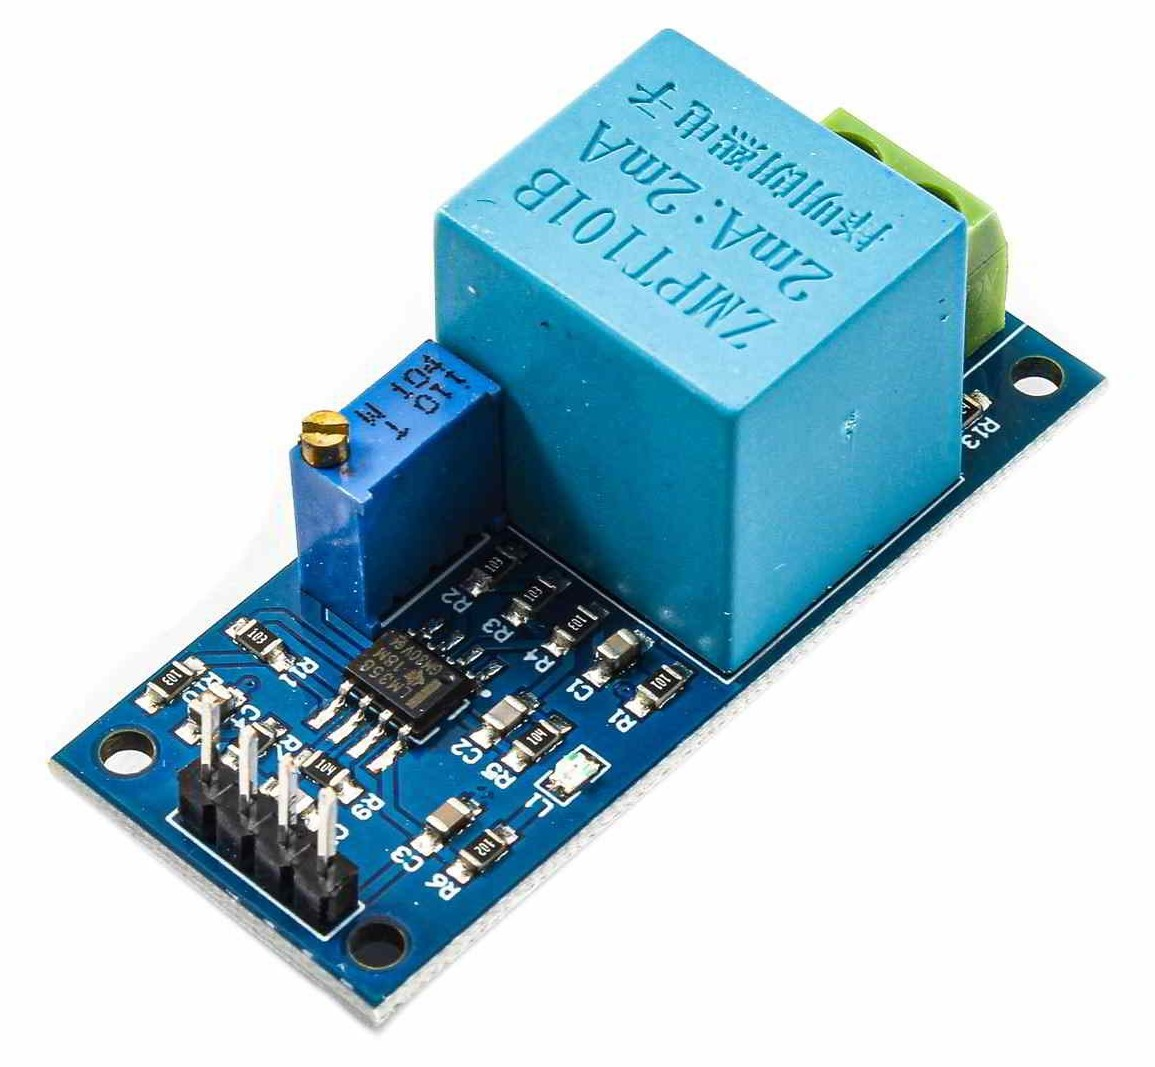
\includegraphics[width=0.4\textwidth]{images/zmpt101b.jpg}
        \caption{Modul se senzorem ZMPT101B~\cite{obrazek_zmpt}}
        \label{modul se senzorem ZMPT101B}
\end{figure}


\subsection{Vložení tabulky}
Tabulka~\ref{tab:example} shrnuje data související s tématem.

\begin{table}[h!]
    \centering
    \begin{tabular}{l l}
        \hline
        \textbf{Parametr} & \textbf{Hodnota} \\
        \hline
        Příklad 1         & 123              \\
        Příklad 2         & 456              \\
        Příklad 3         & 789              \\
        \hline
    \end{tabular}
    \caption{Příklad tabulky shrnující data.}
    \label{tab:example}
\end{table}


\subsection{Příklad parametrického příkazu}
Následuje příklad využití vlastního příkazu \verb|\point|:

\point{Bod 1}Tento bod je důležitý.
\point{Bod 2}Další důležitá informace.
\point{Bod 3}Závěrečné shrnutí.

\sectionbreak

\subsection{Napájení mikrokontroleru a přídavných modulů} 
Z hlediska napájení mikrokontroleru a přídavných modulů bylo nezbytné zajistit stabilní a dostatečný zdroj 
energie. Po zvážení různých možností byl jako nejvhodnější zdroj energie vybrán transformátor (Obrázek~\ref{trafo}), který je schopen převést vstupní elektrický proud na 5V DC s proudem 2A. Tento zdroj by měl být 
dostatečný pro napájení všech nízkoproudových zařízení v rámci prototypu. Dále byl do prototypu integrován 
modulární vstup s konektorem IEC13 (Obrázek~\ref{konektor}), který najdeme u široké škály různých zařízení, 
které najdeme v domácnostech. Tento konektor je navíc vybaven pojistkou a spínačem pro snadné zapnutí a 
vypnutí prototypu.

\begin{figure}[!tbp]
  \centering
  \begin{minipage}[b]{0.3\textwidth}
    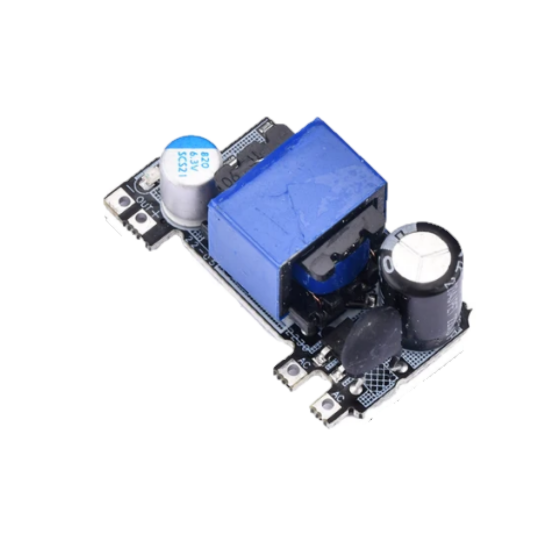
\includegraphics[width=\textwidth]{images/trafo.png}
    \caption{Transformátor~\cite{obrazek_trafo}}
    \label{trafo}
  \end{minipage}
  \hfill
  \begin{minipage}[b]{0.3\textwidth}
    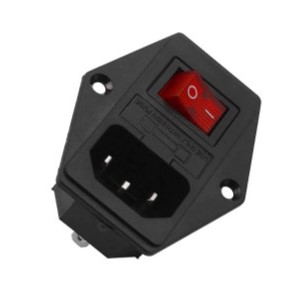
\includegraphics[width=\textwidth]{images/zasuvka.jpg}
    \caption{Konektor IEC13~\cite{obrazek_konektor}}
    \label{konektor}
  \end{minipage}
\end{figure}


\printbibliography[heading=bibintoc,title={Použitá literatura}]

\end{document}
